 \documentclass[conference]{IEEEtran}
\usepackage[utf8]{inputenc}
\usepackage{graphicx}
\usepackage{svg}
\usepackage{todonotes}
\usepackage{mathtools}
\usepackage{algpseudocode}
\usepackage{algorithm}
\usepackage{amsmath}
\usepackage{float}



% correct bad hyphenation here
\usepackage{cite}
\hyphenation{op-tical net-works semi-conduc-tor}

\DeclareUnicodeCharacter{00A0}{~}

\begin{document}
%
% paper title
% can use linebreaks \\ within to get better formatting as desired
\title{Traffic Lane Detection in Urban Environments}


\author{\IEEEauthorblockN{Marin Vlastelica Pogančić}
\IEEEauthorblockA{Karlsruher Institüt für Technologie\\
Karlsruhe, Deutschland\\
Supervisor: Florian Kuhnt}}


% make the title area
\maketitle


\begin{abstract}
%\boldmath
We live in a time of rapid development of autonomous driving systems and the continuous deployment of the same systems in everyday life. This poses a large span of challenges, in order to make the systems reliable and robust in their deployment, much of this robustness relies on the information obtained through sensors from the environment. The pros and cons of different approaches for traffic lane detection will be discussed and the corresponding results compared, with an emphasis on the urban environment, where the challenge of detecting the lanes requires more consideration. 
\end{abstract}



\IEEEpeerreviewmaketitle



\section{Introduction}

As mentioned in the abstract, lane traffic detection in urban environments poses an even greater challenge, there are many reasons for this. One of the main reasons is the cluttered environment, urban environments have many objects, obstacles on the streets which can contribute to the ambiguity of the sensor data. On the other hand, we have many streets in urban environments that don't have lane markings, which means that robust curb detection is also needed to detect the traffic lanes correctly. In chapter II are the lane marking methods discussed. In chapter III are the curb detection methods discussed. 

\subsection{Diverse Approaches}

Diverse solutions for the lane detection problems exist since a long time ago, most of them based on 3D data analysis and pattern recognition. The challenge is to improve the robustness of the detection algorithms using additional context. Therefore, there are some approaches using vehicle tracking to determine the positions of the markings, like proposed in \cite{virtuallane}, that try to use additional context to make the detections more robust and effective. Albeit there are many approaches in this field, the sensor data in use is not so diverse, the driving lane detection is mostly based on stereo-camera imagery and 3D laser sensor data.


\section{Lane Marker Detection}

Lane marker detection is one of the important, if not the most important, challenges in autonomous driving in general. The situation in which the car finds itself will mostly contain environments with traffic lanes denoted by lane markings. Because the environments in which the lanes should be detected are often cluttered, this task is coupled with object detection and prediction methods to make it more efficient. Nowadays the methods for detecting lanes could be divided into two categories: feature-based and model-based methods. The feature-based methods locate the lane-markings using segmentation algorithms whereas the model-based methods use mathematical models to represent the lane. Although the model-base methods achieve impressive results considering their low FPR, they mostly carry high computational costs which unable them to be used in a real-time system.

\subsection{Improved RANSAC Algorithm}

The RANSAC algorithm is the most often used algorithm for lane marking detection. The algorithm is basically an iterative method to estimate parameters of a mathematical model from a set of observed data which contains outliers. In this section will the approach proposed in \cite{ransac} be discussed, which contains a lane marking model-based detection method with an improved RANSAC algorithm.

To achieve a better result in the lane detection step, some image preprocessing is required. The image preprocessing steps that were taken in \cite{ransac} are the following. First of all, a region of interest in the image is chosen. The next preprocessing step is a spatial graying of the image, so the worn out yellow lane markings are better detected. The spatial graying of the image is achieved by 5:4:1 weighted summing of the RGB values, which is proven to be more efficient for determining edges in previous approaches. In addition to the mentioned, a vanishing point of the lanes is added, which can be determined by means of the camera parameters. The last step of the image preprocessing is the denoising of the image. This is achieved by the median filtering method, to meet the real-time requirements.

The most common features used in lane detection are image gradient and edge features. The reason for the preference of these features is their simplicity, which benefits the real-time requirement of the system. Unfortunately these features are also prone to changing lighting conditions. The edge detection algorithm used in this method is the Canny edge detection algorithm.

After the feature extraction part, the next crucial step is lane modelling and lane model parameter estimation. Here comes the trade-off, simple lane models are not able to detect the lanes accurately, for them complex lane shapes (curved lanes) present a problem. On the other hand, the more complex the models are the complexity of the parameter estimation rises and therefore, the computational costs. These points need to be kept in mind when designing a real-time system. For this method, the left and right lane boundaries are described by generalized curves, which has shown good results in the past, in addition, the model takes the planar ground surface and parallel lines constraints.  This model approach is in detail described in \cite{ransac1}. The generalized curve can be described by \ref{eq1}.

\begin{equation}
x = \frac{a}{y-vp_y}+b(y-vp_y) +c
\label{eq1}
\end{equation}

The parameter definitions are as follows: parameter $a$ controls the curvature of the curve, parameter $c$ represents the vanishing point positions, parameter $b$ corresponds to the horizontal positions of the left and right curves - the positions of intersections between the curves and the lowest row of the image, parameter $vp_y$ denotes the vanishing line position in the image and the parameters $x$ and $y$ are the number of the rows and columns of the image. For example, a straight line in the model can be represented when the parameter $a$ is set to 0. 

The parameter estimation of the model is the most important step of the lane detection process, this is where the RANSAC algorithm comes into play, a more detailed explanation of the RANSAC algorithm is available in \cite{ransac2}. The RANSAC algorithm can adapt to the
complex conditions of lane estimation of model parameters
and it does not need training process compared to the Hough
transform and template matching method.

The lane feature points extracted by the Canny method contain a lot of noisy points for various reasons as damaged road surface or varying lighting conditions for example. This makes it very difficult to calculate the lane model parameters correctly. The improved RANSAC algorithm has a process as follows.

\begin{algorithm}
\caption{The improved RANSAC algorithm}
\label{alg1}
\begin{algorithmic}[1]
\State Initial lane model parameter vector $Mod=NULL$, iterator $i=1$, get lane boundary feature points set $P$, inlier points set $I=NULL$, $Modbest=NULL$, $S=0$. \linebreak
\State Random select $n$ ($n=3$) points from $P$ (these points should be located in different rows of the image), calculate $Mod$ by these points.
\State For any point $p_i(y_i,x_i)$ $p_i \in P $, if $Dist(p_i)<D_{threshold}$, add $p_i$ to inlier points set $I$.
\State If $number(I) < Num_{threshold}$ or $Mod$ doesn't meet the constraints, $P=P-I,I=NULL$, goto step 2).
\State Recalculate $Mod$ by function $LeastSquareFit(I)$, If $Score(I)>S, S=Score(I), Modbest=Mod, P=P-I, I=NULL, i++$
\State If $i < numIterations$, go to step 2
\end{algorithmic}

\end{algorithm} 

In the algorithm \ref{alg1} is the vector $Mod = [a,b,c]$, function $Dist(p_i) = |x_i - \frac{a}{y_i - vp_y} + b(y_i - vp_y)+ c|$. $D_{threshold} = 1$, $Num_{threshold} = 12$ and the function $Score(I) = \sum_{p_i \in I}t(p_i)$ 
$t(p_i) \in [0,1]$ if $Dist(p_i) < 1, t(p_i) = 1$, else $t(p_i)=0$.

\begin{figure*}
	\centering
    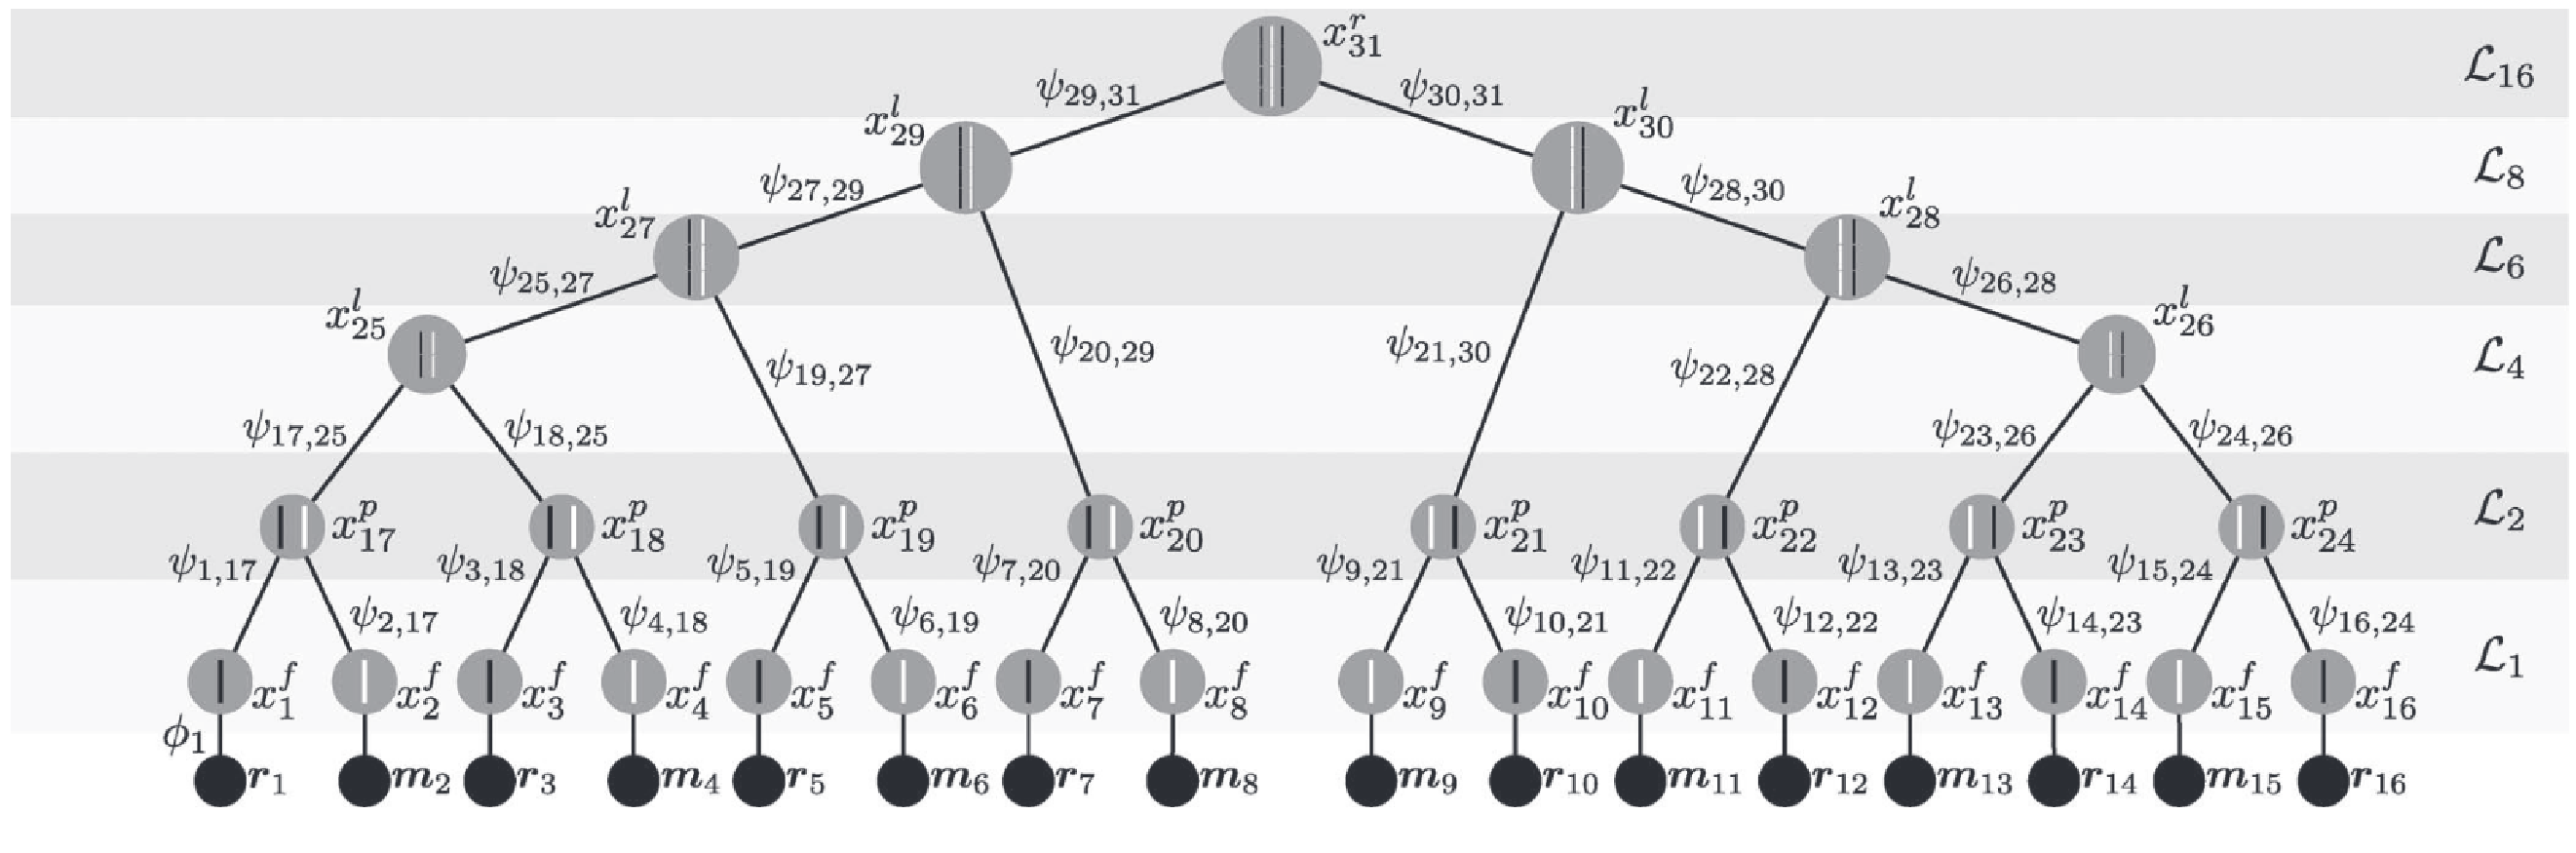
\includegraphics[scale = 0.4]{pictures/tree.pdf}
	\caption{CHM of a two-lane road. This figure shows the factorization of the joint probability distribution in (2) using an undirected graphical model. Hidden random variables are depicted in gray and symbols illustrate their type, i.e., features, patches, lanes, and multilane roads. Observable variables are shown in blackand dependencies between random variables are highlighted using edges. \cite{lanesystem}}
	\label{fig10}
\end{figure*}

The $LeastSquaresFit(I)$ is a function which takes points of set $I$ and fits the lane model using a least squares method.



\begin{table}[]
\centering
\caption{Improved RANSAC method evaluation}
\label{eval1}
\begin{tabular}{c c c}
\hline
Datasets & TPR & FPR \\
\hline 
\\
1 & 96.37\% & 3.17\% \\
2 & 97.24\% & 25.39\% \\
3 & 94.64\% & 7.23\% \\
4 & 94.73\% & 3.85\% \\
\end{tabular}
\end{table}


\begin{figure}[ht]
	\centering
   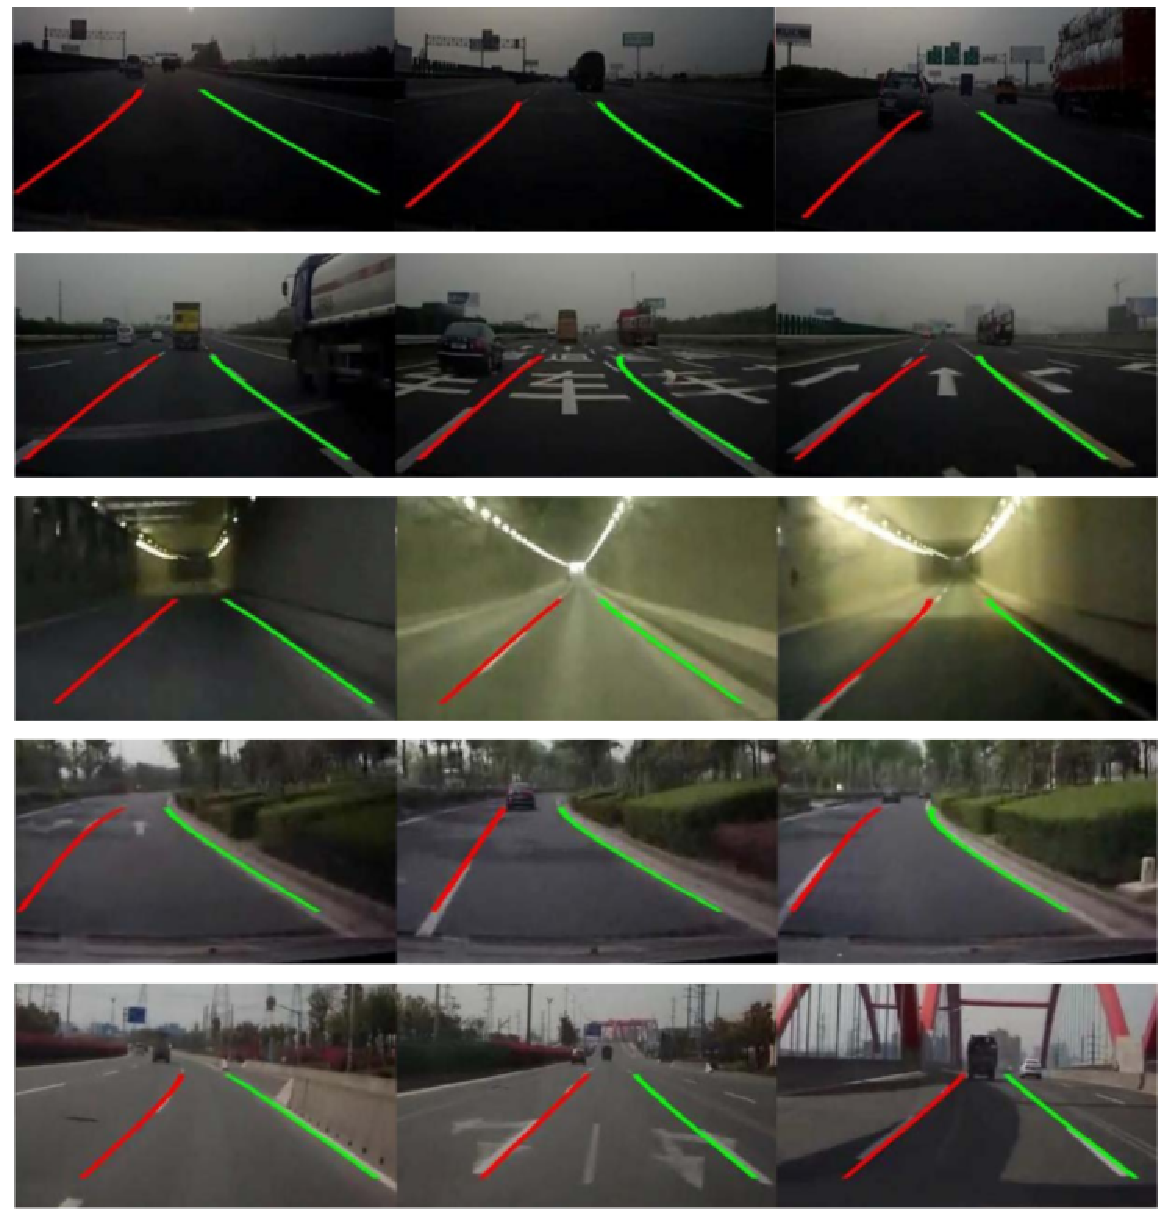
\includegraphics[scale = 0.5]{pictures/good_detections.pdf}
	\caption{Good detection results \cite{ransac}}
	\label{fig5}
\end{figure}


\begin{figure}[H]
	\centering
    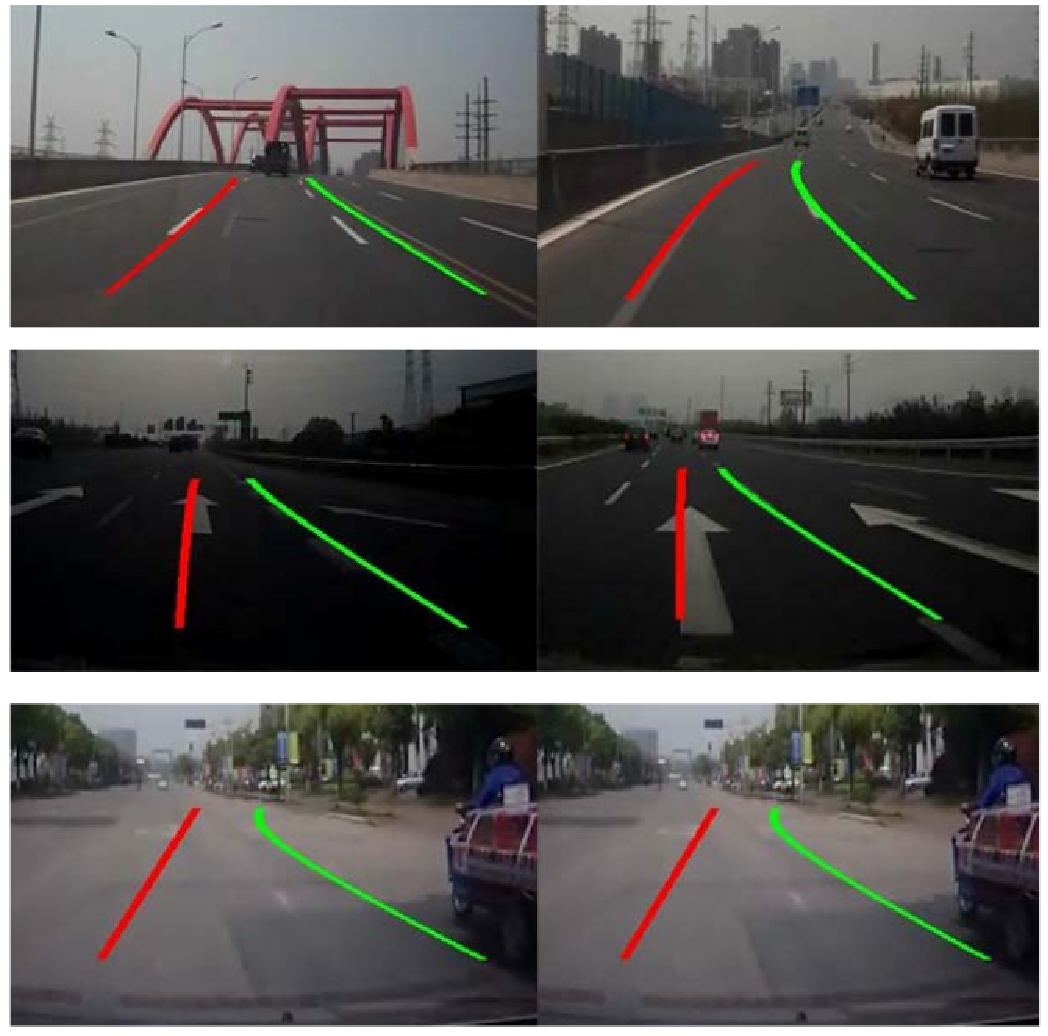
\includegraphics[scale = 0.5]{pictures/bad_detections.pdf}
	\caption{Bad detection results \cite{ransac}}
	\label{fig6}
\end{figure}



The results presented in table \ref{eval1} are obtained from the Caltech lane dataset. Unfortunately, this method clearly has problems with signs on the road, which can be seen in figure \ref{fig6}.

\subsection{Tree Based Graphical Model}

In this section an approach will be discussed, that is based on a tree based graphical model of the road \cite{lanesystem}. The purpose of the tree model is to capture the way the joint distributions over random variables can be decomposed into a product of factors. The end goal is the development of efficient inference algorithms. The example of the tree based structure for a multilane road can be seen in figure \ref{fig10}.
The nodes on the lower level represent a recursive decomposition of the root object into parts and subparts, this enables the dividing of the perception problem into subproblems that are easier to solve. One of the shortcomings of this approach is that it assumes a flat road surface. The model of the scene is made in the vehicle coordinate system, located at the center of the rear axis. 

The tree is encoded by an undirected structured graph. The nodes correspond to three disjoint sets of variables $x \cup m \cup r$.  Each $x$ variable represents a part or a subpart of the multilane road, this is a hidden variable. The $m$ and $r$ variables correspond to the lane marking features and the road edge features. The edges between pairs of hidden variables define spatial constraints, which encode the dependencies between neighboring hidden variables by means of conditional spatial distributions. Edges between hidden and observable random variables encode observation potentials.The details of the probability distribution factorization can be found in \cite{lanesystem}

The leaves encode feature variables with associated observations, two of the observed features define a local driveable area referred to as patch, which form the second level of the tree. The figure \ref{fig11} illustrates that each patch is defined by a left and right lane boundary feature.

\begin{figure}[H]
	\centering
    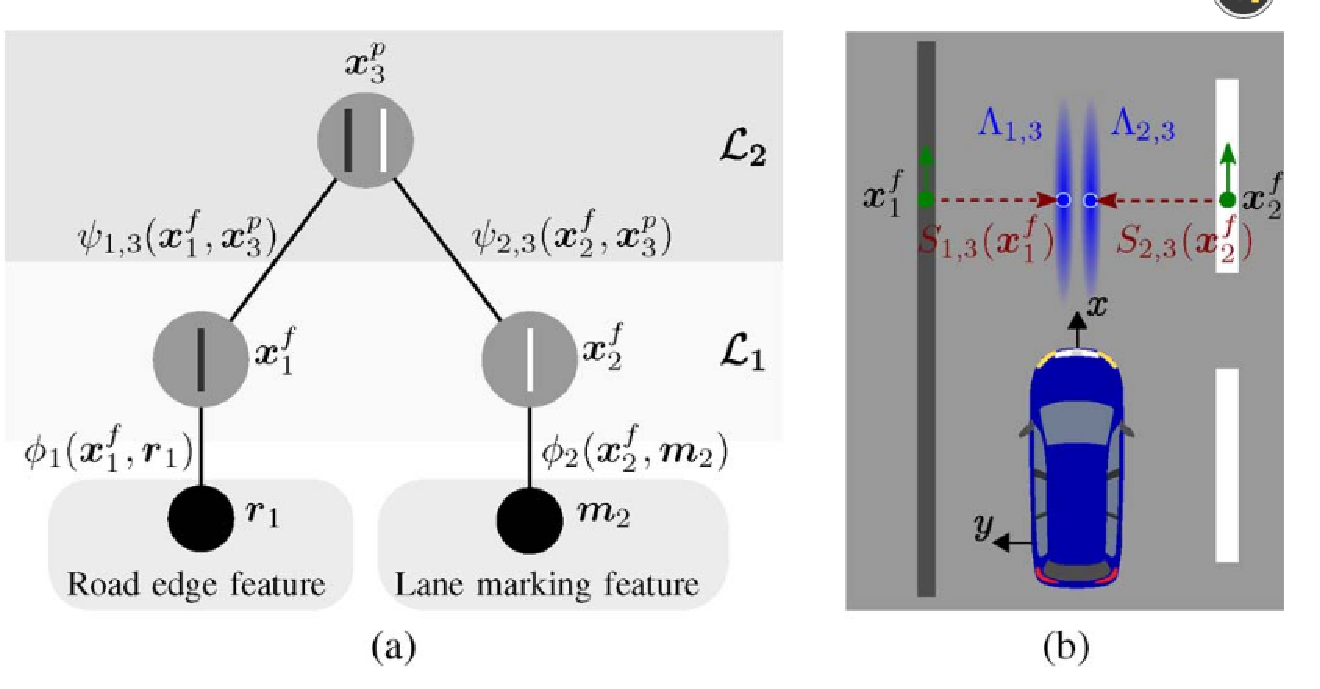
\includegraphics[scale = 0.4]{pictures/patch.pdf}
	\caption{CHM of a patch and illustration of the modeled spatial constraints.(a) Patch is decomposed into a left and a right lane boundary, which are directly observable. (b) Illustration of the modeled spatial constraints, where spatial uncertainties are illustrated by showing 2-D Gaussian distributions, where dark colors correspond to more likely locations.\cite{lanesystem}}
	\label{fig11}
\end{figure}

The constraints between feature variables $x^f_i$ and patch variables $x^p_i$ are modelled using weak spatial constraints. 

\begin{equation}
\label{eq5}
S_{ij}(x_i^f) = \begin{bmatrix}
x_i \\
y_i \\
\vartheta \\
\end{bmatrix}
+ \begin{bmatrix}
\frac{1}{2}sin(\vartheta_i) & 0 & 0 & 0 & 0 \\
0 & -\frac{1}{2}sin(\vartheta_i) & 0 &0 & 0 \\
0 & 0 & 1 & 0 & 0 \\
0 & 0 & 0 & 1 & 0 \\
0 & 0 & 0 & 0 & 1 \\
\end{bmatrix}
\begin{bmatrix}
\upsilon_{w_p} \\
\upsilon_{w_p} \\
0 \\
\upsilon_{w_p} \\
\upsilon l_{v_p} \\
\end{bmatrix}
\end{equation}

\begin{figure*}
	\centering
    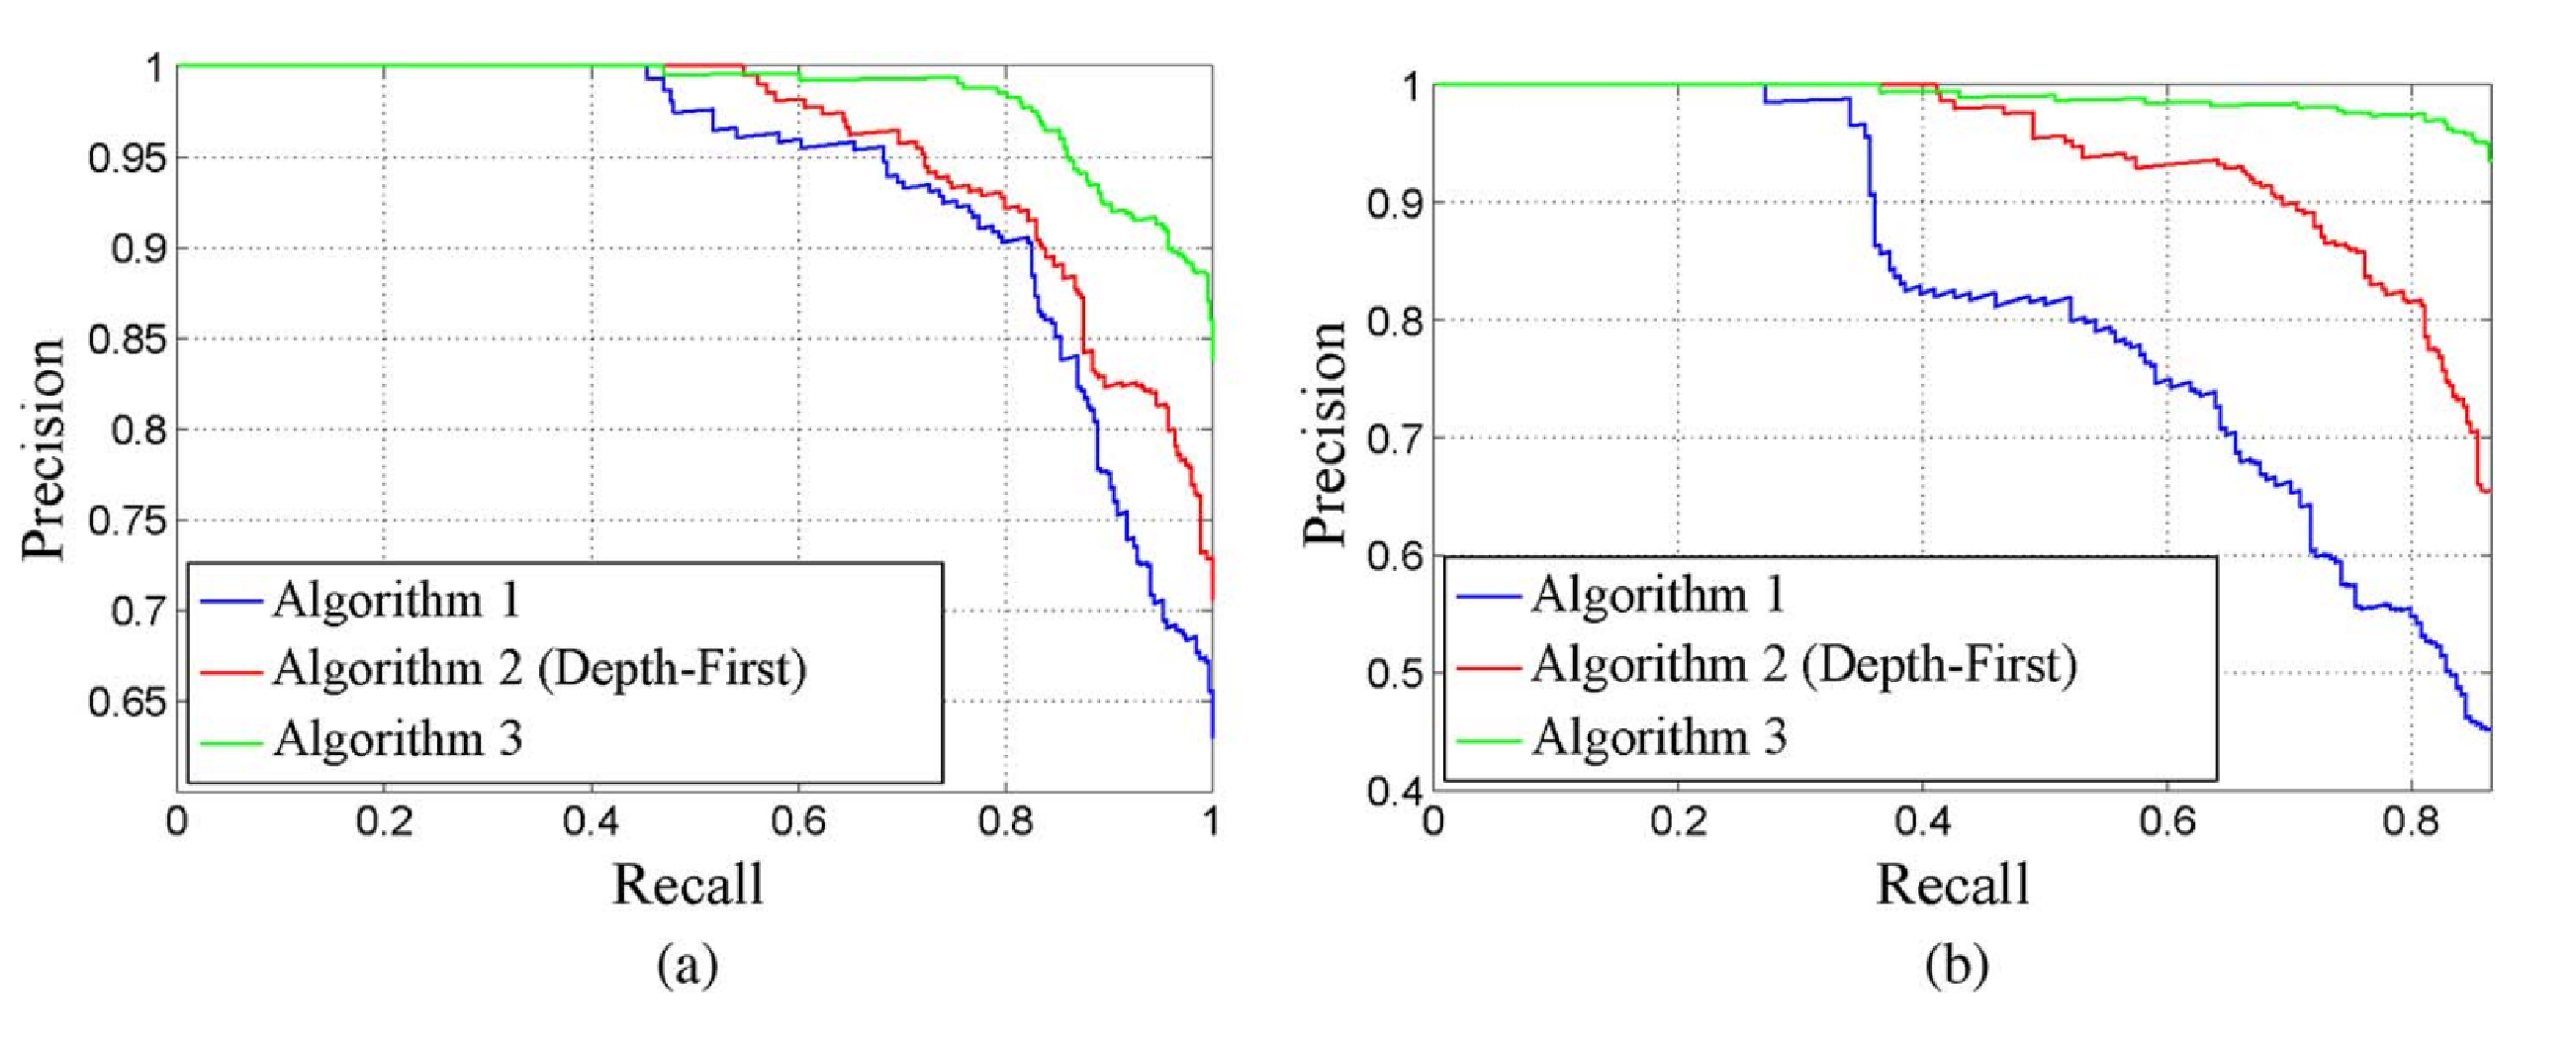
\includegraphics[scale = 0.4]{pictures/roc.pdf}
	\caption{Precision–Recall curves for (a) highway scenarios and for (b) rural scenarios. Results are computed using different algorithms and evaluated against theground truth\cite{lanesystem}}
	\label{fig12}
\end{figure*}


The transformation in \ref{eq5} returns the predicted location of the variable $x_j^p$ based on the expected lane width $\upsilon_{w_p}$ and the state of variable $x_i^f$. 

The next higher levels of the tree consist of lanes of increasing length, lanes are defined as a composition of individual patches. That means that the lanes are represented by a polygonal path with piecewise constant orientation and width. The length of a lane is defined as a sum of the euclidean distances between subsequent lane elements. Spatial constraints between pairs of lane variables are expected to predict the expected location of the subsequent lane element:
\begin{equation}
S_{ij}(x_i^l) = \begin{bmatrix}
x_i \\
y_i \\
\vartheta_i \\
w_i \\
\end{bmatrix} +
\begin{bmatrix}
cos(\vartheta_i) & 0 & 0 & 0 \\
0 & sin(\vartheta_i) & 0 & 0 \\
0 & 0 & 1 & 0\\
0 & 0 & 0 & 1 \\
\end{bmatrix}
\begin{bmatrix}
\upsilon l_p \\
\upsilon l_p \\
0 \\
0 \\
\end{bmatrix}
\end{equation}

The $\upsilon l $ is the constant patch length defining the segmentation of the center line, which allows the control of the complexity of the inference. 

The problem of modeling the spatial constraints is the center discussion in this approach. This is the consequence of the model, the spatial constraints determine the complexity of the model and therefore its applicability in real-time systems. 

The task of lane and road perception is the equivalent of computing the marginal posterior distribution of all or a subset of the hidden variables in the graphical model, which can efficiently be performed with Belief Propagation, for which a detailed explanation can be found in \cite{lanesystem}.

The results of this method are presented in an ROC graph form, which can be seen in figure \ref{fig12}. The graph shows the results obtained based on 3 different approaches to tree searching.

\section{Road Curb Detection}

One of the more important tasks in an urban environment is curb detection. The reason for this is that many streets in an urban environment are small streets without lane markings. In order to fully function in an urban environment, autonomous vehicles have to solve this problem in an appropriate manner also. In this chapter will the different approaches to solving this problem be mentioned.  

\subsection{Elevation Mapping Techniques With Stereo Camera}

In this chapter will an approach suggested in \cite{stereo} be explained. The approach, as the name suggests, is based on using elevation maps. By means of these maps can the most probable paths be calculated. The position accuracy that was able to be achieved is about 10 cm and an height error of about 1.5 cm, tested in real-time.

The sensor used primarily in this approach is the stereo camera, where the output of the stereo camera are two intensity images and one disparity image. For the ego motion is the inertial measurement unit used. 

The first step that is to be made is to take the disparity image and generate a position 3D point cloud from it in the sensor coordinate system. This generated point cloud finds itself in the sensor coordinate system at the beginning, the next step is to transform this point cloud into the map coordinate system after the ground pixels had been detected. Thereafter is important to use the ego motion estimation. 

The ego motion estimation is used to estimate the ego motion of the vehicle between two timestamps. The DEM model used in this approach is based on a 2.5-D map described in \cite{bewegung}. It accumulates of the stereo camera in the Euclidean space using temporal integration. One cell in the map is of the size 20 x 20 cm and has a one dimensional Kalman-Filter which estimates the height of the cell. In each prediction step is the cell height adjusted according to the ego motion of the car, for the correction step is the Kalman-Filter updated with the sensor measurements. 

The detection approach is as follows. The static and dynamic objects lead to value spikes in the DEM, whereby the dynamic objects need to be removed, in order to detect the curbs. The dynamic objects are detected with a laser scanner and removed from the point cloud generated from the stereo camera.The rest of the points are divided into ground points and object points. The ground detection algorithm assumes steadily growing x values in the sensor coordinate system, when the disparity image columns are considered. If the x values are steadily growing, then it can be assumed, that ground is in front of the car, otherwise this assumption cannot be made. To compensate the effect of the outliers, the mean value of two consecutive columns with 3 pixels each is calculated.

What also must be considered are the mapping techniques which also have an effect on the performance, since these are not the central aspect of this paper, all of them are mentioned and analysed in \cite{stereo}. The mapping techniques used in \cite{stereo} are the following: vehicle body based mapping, global mapping and road surface based mapping. 


\begin{enumerate}
\item Vehicle body based mapping
\begin{itemize}
\item Transforms the point cloud without the use of angles dependent on the ego motion
\item Compensates every cell by its individual compensation value depending on the cell position relative to the origin of the coordinate system.
\item Additionally to the angles and the ego motion uses the global pitch and yaw rate and the change of the body height compared to the ESC coordinate system.
\item Does not use estimation of road surface.
\end{itemize}

\item Global mapping
\begin{itemize}
\item Every cell has to be compensated by the same value.
\item The highest demands on ego motion estimation, depends on the same angles as BBM and additionally uses the global pitch and roll. angles.
\item Does not use estimation of road surface.
\end{itemize}


\item Road surface based mapping
\begin{itemize}
\item Requires estimation of the road surface and calculation of the relative height values
\item Point cloud transformation computationally intensive
\item Simple ego motion compensation, shift in x- and y-direction and compensation of the yaw angle
\item Uses angles to the local street and the two-dimensional ego motion in the ESC coordinate system  for coordinate transformation and ego compensation of the map.
\item Has lower information value, it only contains relative heights to the local surface estimation. 
\item Uses estimation of road surface to calculate relative heights. This means that this mapping technique is mainly influenced by the road estimation.
\end{itemize}
\end{enumerate}


The road curb is represented by a polygonal chain, this chain consists of supporting points and the connections between these supporting points. Every point contains a 2D position and the road curb height at its position. The chain consists of supporting points and the connection between these supporting points. Every supporting point contains a 2D position of the road curb height at its position ass seen in figure \ref{fig7}. 


\begin{figure}[ht]
	\centering
  	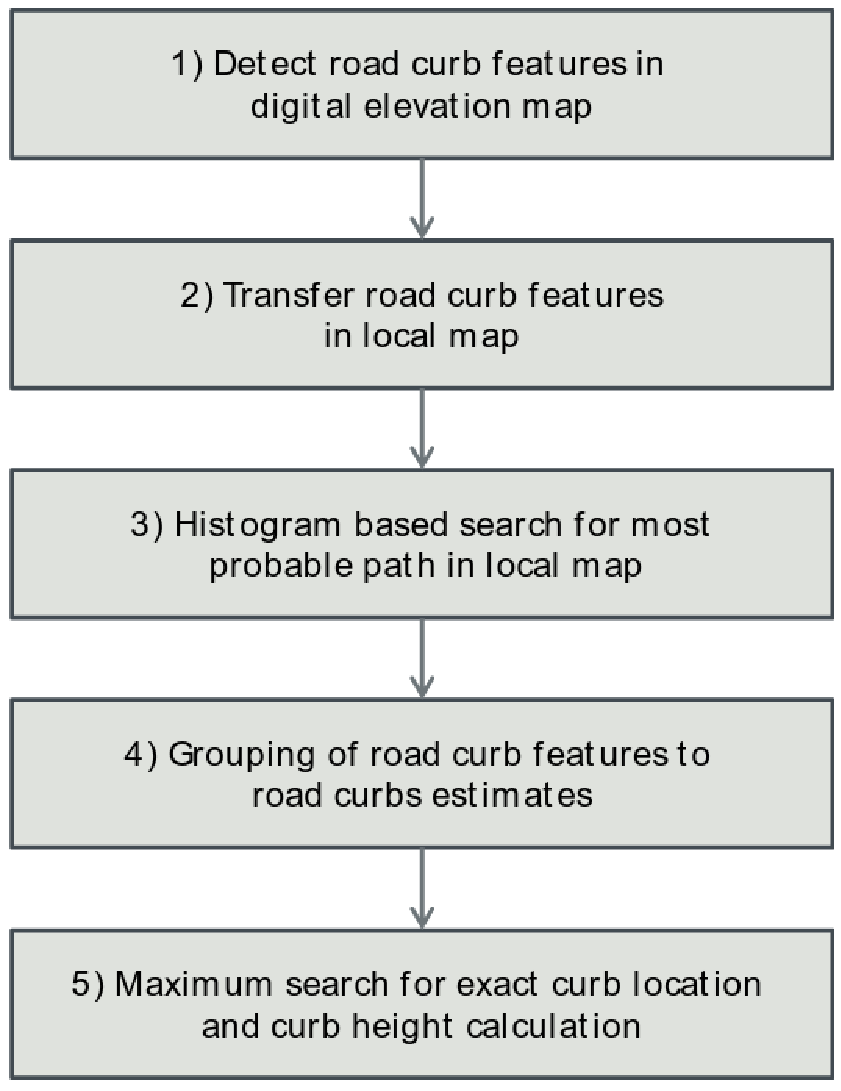
\includegraphics[scale = 0.5]{pictures/detection_process.pdf}
	\caption{Detection process}
	\label{fig8}
\end{figure}



The first step at road curb detection is the road curb feature extraction. This is achieved by applying an edge-detection algorithm on the DEM to find cells with a jump in the neighbouring height values, which might be caused by a road curb. Only cells with a minimal number of updates are considered, because less updates means more noise. A Sobel operator is used for the edge detection an the result is normalized, if the normalized result finds itself within a range, then a road curb feature is found. 



\begin{figure}[ht]
	\centering
    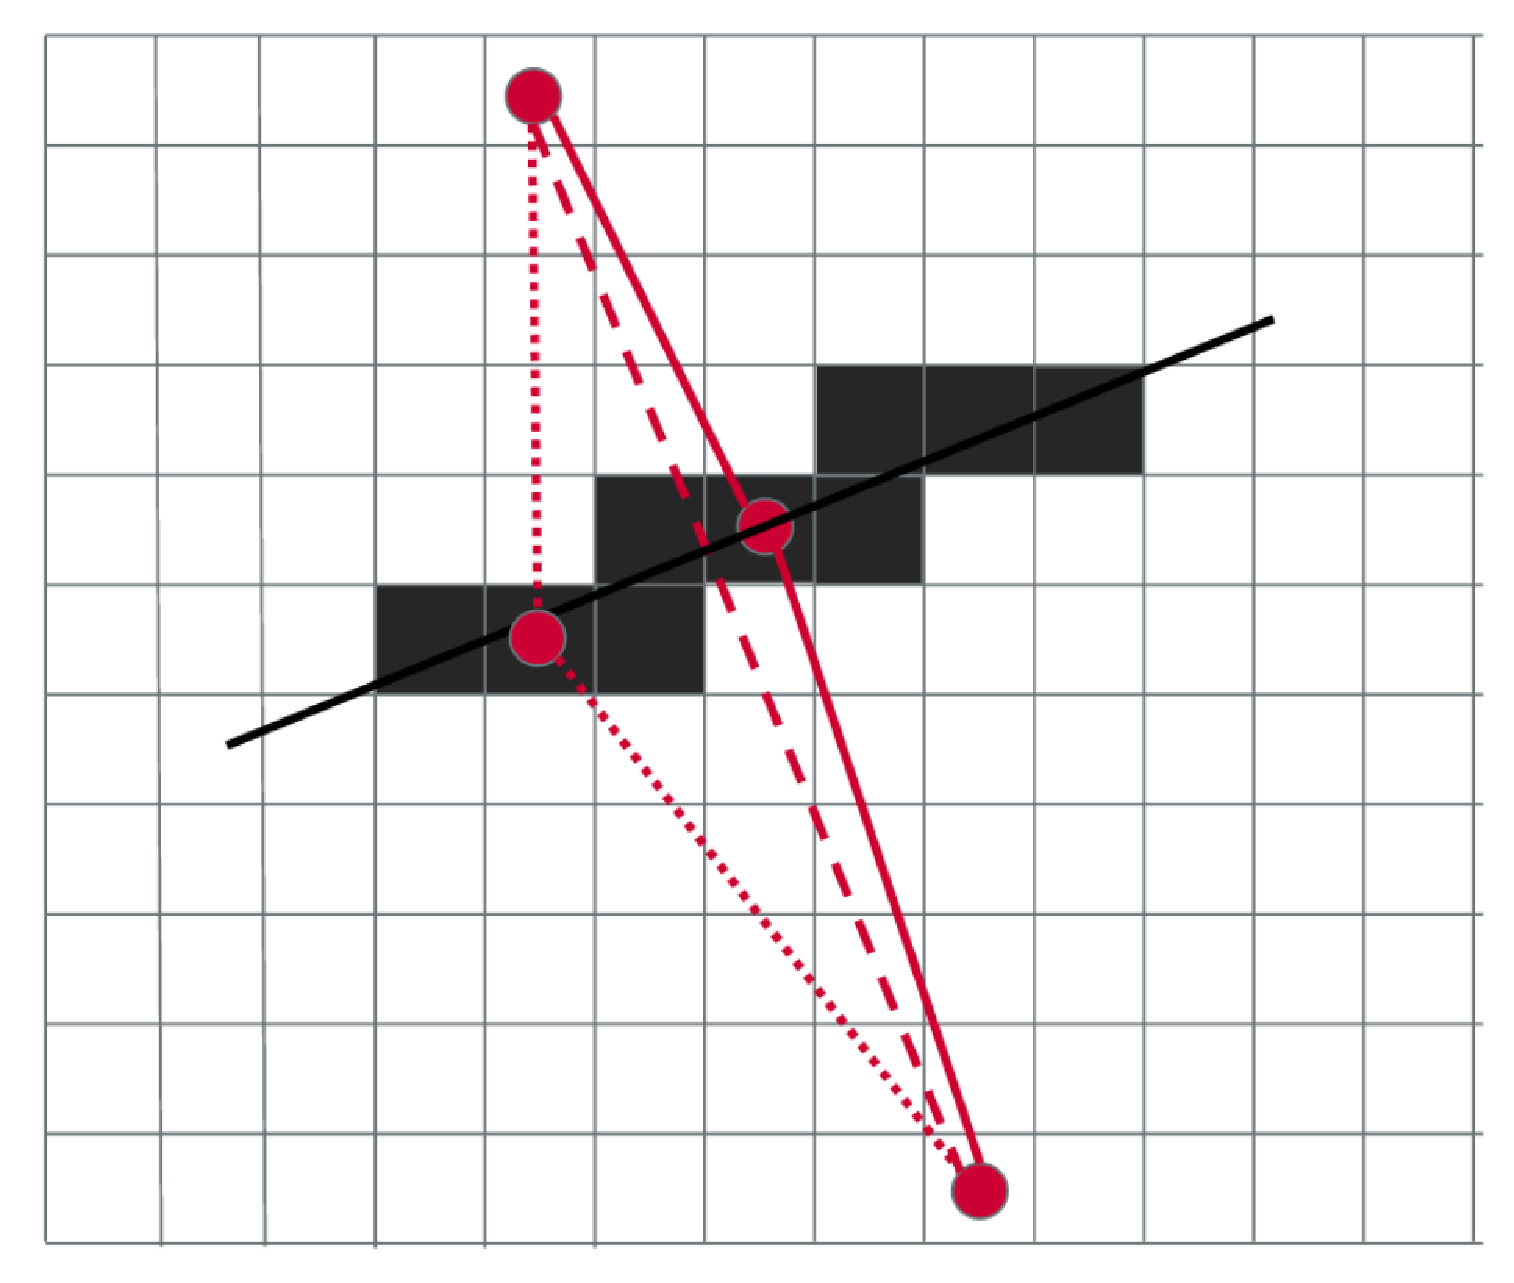
\includegraphics[scale = 0.3]{pictures/polygonal_chain.pdf}
	\caption{Polygonal chain - red points: supporting points of road curb polygonal chain ;red line: original link between supporting points; black line: perpendicular line to the connection of supporting points used for maximum search; red dotted line: new link between supporting points after maximum search \cite{stereo}}
	\label{fig7}
\end{figure}


In the next step the features are registered in a second map with the size of the region of interest and a lower resolution.There must be a minimum of features in one of the low resolutions cells to be marked as a curb cell, because a road curb is not a singular feature like a reflector post used for road boundary detection. By building histograms of road curb features perpendicular to the driving direction the most probable path is determined. To build the polygonal chain the minimal distance approach is used,which considers the closest features to the most probable path as the road curb. In general the road curb is the closest boundary to the path visible in an elevation map. The output of the road curb detection algorithm are polygonal chains for both sides of the vehicle.

After the above steps had been completed, now a maximum search and calculation of curb height can take place, to enhance the position accuracy of the road curb.The height differences are built using the original values in the digital height map as seen in \ref{eq2}.

\begin{equation}
d_{c,l} = h_{c,l + 1} - h_{c,l -1}
\label{eq2}
\end{equation}

 Here is an approach proposed by Hoffman in \cite{hoffmann} to determine the maximum point with a subcell accuracy:



\begin{equation}
\label{eq4}
w = \frac{d_{c,max-1} - d_{c,max+1}}{2(d_{c,max+1} - 2d_{c,max} + d_{c,max-1})}
\end{equation}
The supporting point for the polygonal chain is moved to the position found by this maximum search strategy. As curb height the highest difference value $d_{c,max}$ is used. 


There is no FPR/TPR evaluation offered for this method, but a speed evaluation was done in comparison between different mapping tehniques.

\begin{table}[H]
\centering
\caption{Method speed evaluation}
\begin{tabular}{| c | c | c | c |}
\hline
Tasks & RSBM & GM & BBM \\
\hline
3D Point Cloud Generation & 8.32 ms & 5.36 ms & 5.38 ms \\
\hline
Ego Compensation and Map Update & 7.51 ms & 7.44 ms & 8.39 ms \\
\hline
Road Curb Detection & 3.73 ms & 3.66 ms & 3.72 ms \\
\hline
Sum & 19.55 ms & 16.46 ms & 17.49 ms \\
\hline
\end{tabular}
\end{table}

\subsection{Laserscanner Based Road Curb Detection}

In this section a method proposed in \cite{lidar13} using a laser scanner to detect road curbs will be described. The argument for using laser scanners instead of stereo cameras is that the laserscanner provides more accurate data. Some methods have been developed, that use sensor fusion with the stereo camera to overcome this precision lacking. Unfortunately these methods produce a big overhead in the data processing step, which makes a big difference in an autonomous vehicle, because it is a real-time system.

For testing this method, the equipment proposed in \cite{lidar13} is the following. For road curb detection, a multipurpose laserscanner is used. For the ego motion estimation a low cost inertial measurement unit is used in combination with the standard wheel speed sensors and chassis lift sensors. 

The road curb detection pipeline is shown in \ref{fig1}. As the figure shows, the detection is split into 3 modules. In the first module is used for for the road curb feature extraction and labelling. The detected road curb candidates have to be accumulated over time, so they are stored into the road curb map, where they undergo ego motion compensation. In the last module uses the temporal filtered parameters stored in the cells of the road curb map to group the road curb candidates into road curbs. In the end, the road curbs are represented as polygonal chains.  

\begin{figure}[ht]
	\centering
    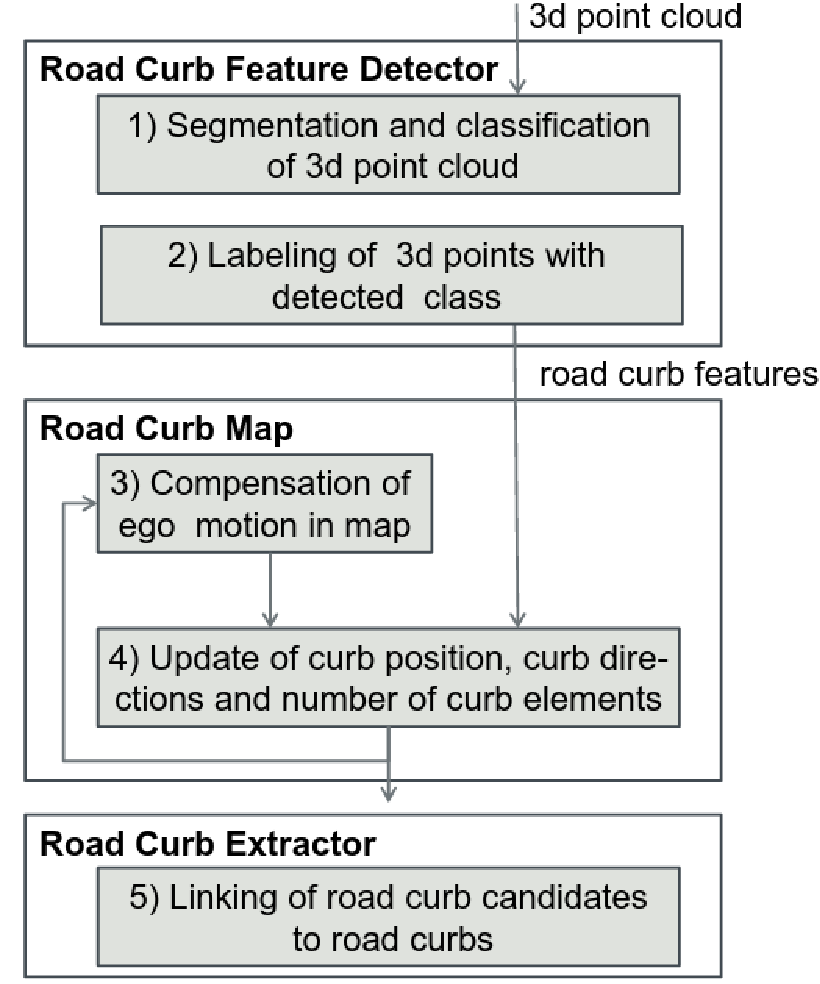
\includegraphics[scale = 0.5]{pictures/system_structure.pdf}
	\caption{System structure \cite{lidar13}}
	\label{fig1}
\end{figure}
  
At the point of detecting road curb features, three approaches can be used: segmentation using iterative end point fit and classification of segments, hierarchic segmentation and classification of segments, segmentation using regression lines and classification of segments.

The IEPF algorithm described in this section is a well known segmentation algorithm. In this method, the input to the algorithm is the orthogonal projections of the 3D points on the y-z plane. The start and end point of the scan line are connected and the distance to the straight line is calculated for each point, as shown in \ref{fig2}. The measurement points are split into two segments at the point with maximum distance, the circled point in \ref{fig2}, if it exceeds a predetermined threshold. This takes place for every generative segment iteratively, till there are no points that cross this threshold. For each segment that contains the minimum number of points, the angle $\alpha_S$ between the regression line of the segments, the average height and the variance of the height values is being calculated. The segments are classified into four classes: road curb, object, ground and street. This method assumes that the segments containing the central channels of the scan lines is a street. After that, the process continues by going in both direction of the scan line and classifying the object segment with a object classification algorithm. For the segments not labelled as objects, an angle between that segment and the last found street segment is calculated. If this angle $|\alpha - \alpha_S|$ is greater than a threshold $T_{\alpha,1}$, the segment is marked as a road curb. If the angle is greater than $T_{\alpha,2}$ but lower than $T_{\alpha,1}$, or the difference to the height of the neighboring lane segment $|h - h_S|$ is lower than $T_h$ or the difference in variance $|\sigma - \sigma_S|$ is above $T_\sigma$, then the segment is marked as ground. The variance criterion is used to distinguish the streets in unstructured environments, with a lot of gravel and grass for example. If none of these criteria are met, then the segment is classified as a street segment and is used for further evaluation of segments. 

\begin{figure}[ht]
	\centering
   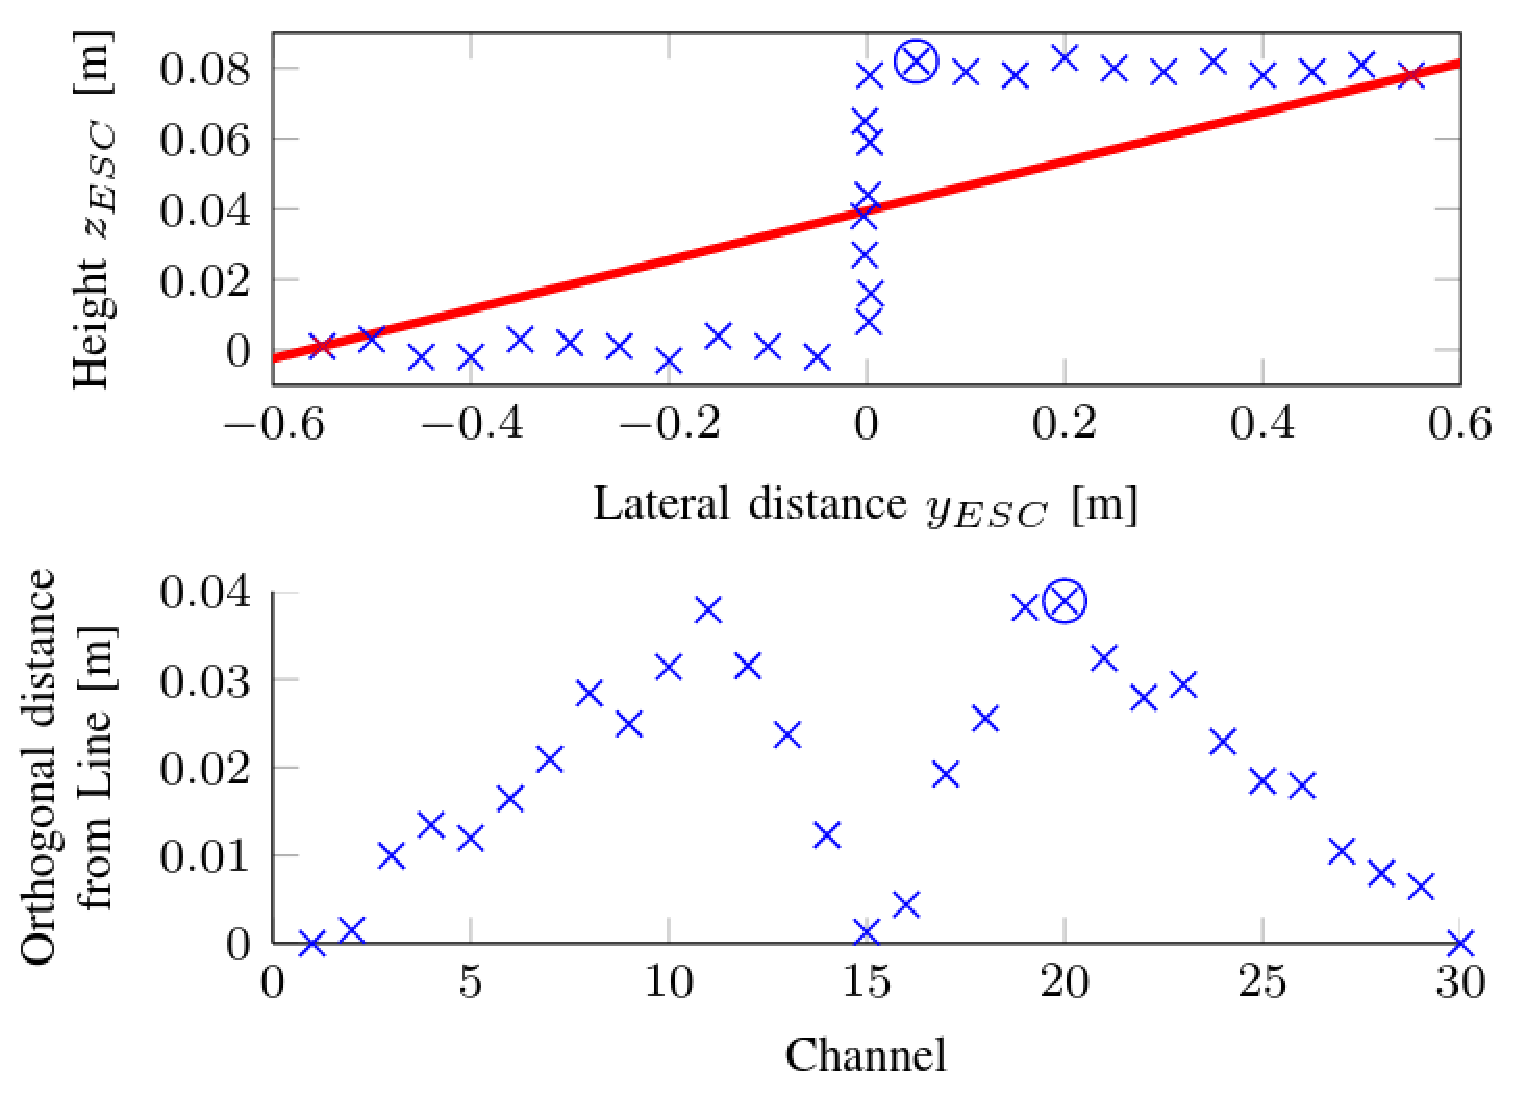
\includegraphics[scale = 0.35]{pictures/iepf.pdf}
	\caption{The IEPF segmentation method  \cite{lidar13}}
	\label{fig2}
\end{figure}
 

Another possible approach for segmentation is segmentation using regression lines. For every measurement point a forward and a backward regression line is calculated containing n points before or after the measurement point. The regression lines are calculated in the z-channel-space.  In all adjunct points with an intersection angle exceeding a certain threshold a maximum search regarding the intersection angle is conducted. At the maximum, a segment is terminated. The classification steps are performed in the y-z-space again as described for the IEPF algorithm. As the regressions lines are build with only a few measurement points this detection algorithm is sensitive to outliers int he data set? This segmentation method is shown in \ref{fig3}

\begin{figure}[H]
	\centering
  	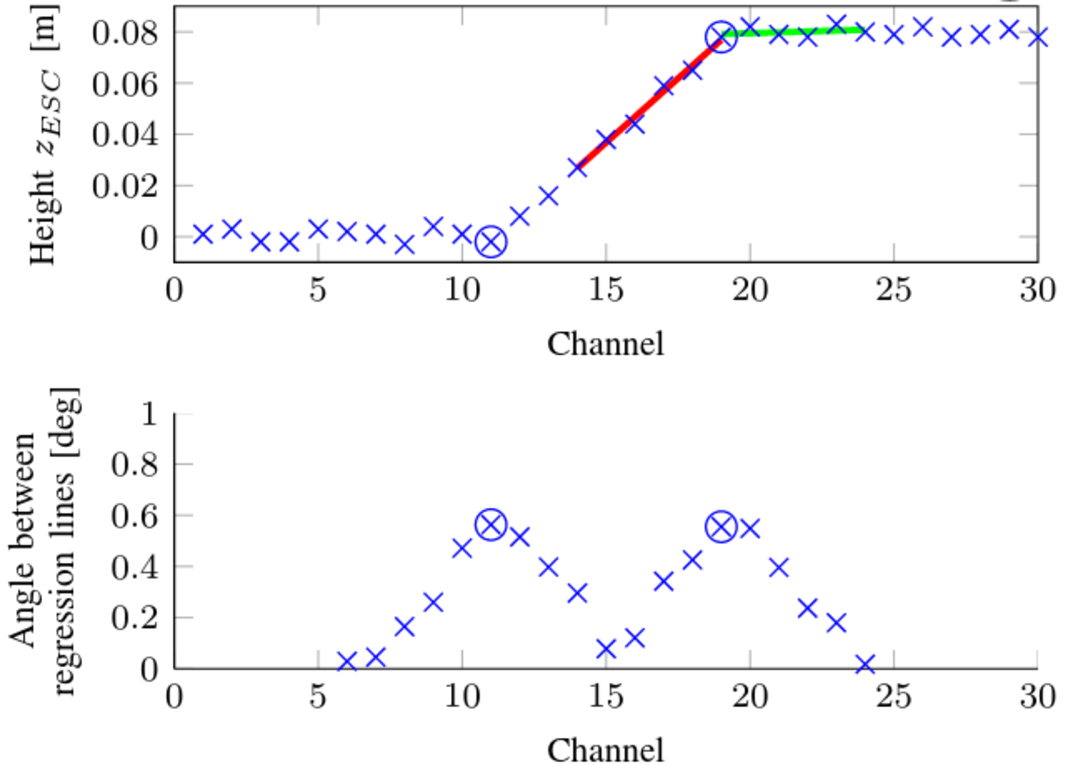
\includegraphics[scale = 0.5]{pictures/iepf2.pdf}
	\caption{Regression lines segmentation method  \cite{lidar13}}
	\label{fig3}
\end{figure}

The final segmentation method considered is the hieararchic segmentation and classification of segments. The segments are built pairwise from neighbouring height values. Two neighbouring segments are merged if the standard deviation of the height values in relation to the calculated regression line of the merged segment is below a certain threshold. This is processed in a pyramid procedure until a new segment does not fulfill the described variance criterion.This process is shown in \ref{fig4}

\begin{figure}[H]
	\centering
 	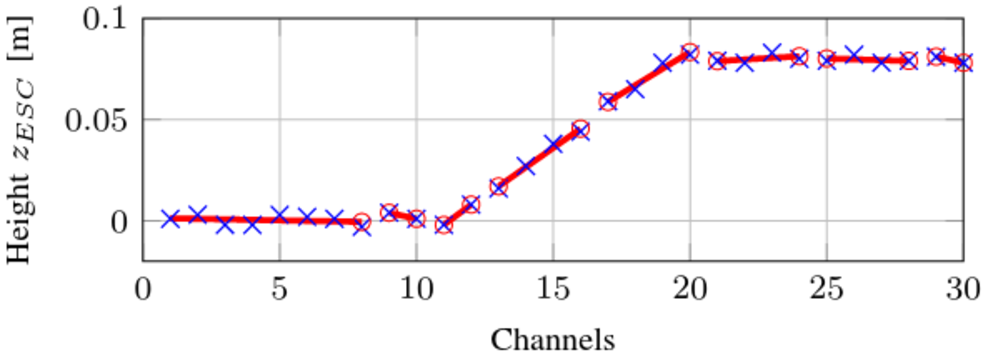
\includegraphics[scale = 0.55]{pictures/iepf3.pdf}
	\caption{Hieararchic segmentation method  \cite{lidar13}}
	\label{fig4}
\end{figure}

The cells of the grid based road curb map contain a local description o the road curb based on a linear model. Each cell contains the model parameters center point $(x^C, y^C)$ and direction $d = (1, \beta_1)^T$, and additionally the number of cell updates n.The model parameters are updated with every curb feature lying in the cell. Of course this is not enough to achieve a precise road curb estimation so the centers of the road curbs are estimated within the cell.

The larger the cell is, the better the computation time and memory consumption. Large cells are good for straight road curbs, but smaller cells are better for road curbs with complex geometry.

For every new measurement frame an additional step is necessary to compensate the ego motion between two measurement time stamps(reference). 

The road curb extraction takes place in the road curb extraction module. The module uses the model parameters to build chains of road curb candidates. To identify the most relevant curb chains, an estimated central line of the current lane is used, as shown in \ref{fig5}



\begin{figure}[H]
	\centering
  	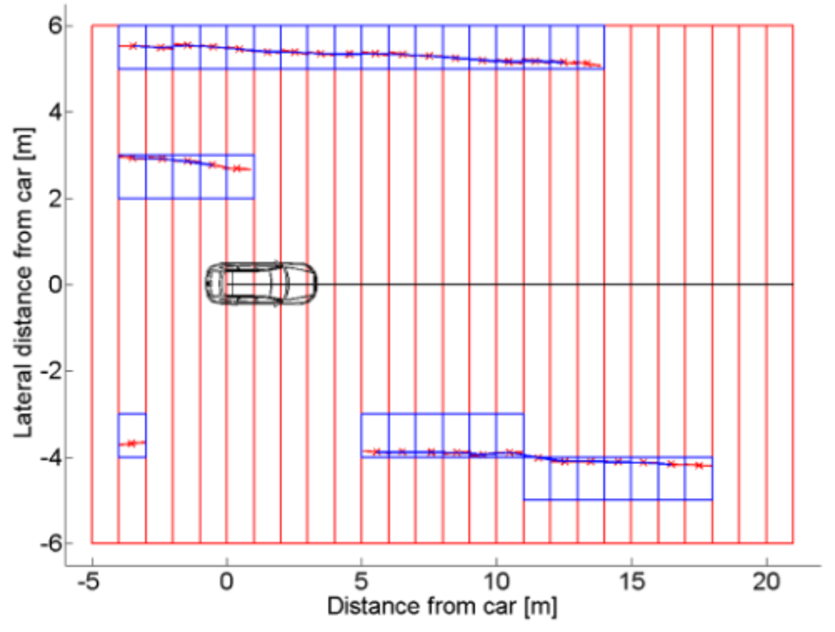
\includegraphics[scale = 0.4]{pictures/extractor.pdf}
	\caption{Data structure of the road curb extractor (blue boxes: road curb candidates with center point (red x) and direction (red line); red boxes: groups or road curb candidates; black line: estimated central line of current lane;blue line: road curb segments) \cite{lidar13}}
	\label{fig5}
\end{figure}


The results obtained with this method are presented in \ref{tab1}.

\begin{table}[]
\centering
\caption{FPR and TPR Evaluation}
\label{tab1}
\resizebox{\columnwidth}{!}{\begin{tabular}{lllllll}
\cline{1-7}
\multicolumn{1}{l}{Methods} & \multicolumn{1}{l}{Curb HR} & \multicolumn{1}{l}{Curb FPR} & \multicolumn{1}{l}{Object HR} & \multicolumn{1}{l}{Object FPR} & \multicolumn{1}{l}{Street HR} & \multicolumn{1}{l}{Street FPR} \\ \cline{1-7} 
IEPF                         & 38.9\%                       & 3.3\%                         & 93.4\%                         & 0.9\%                           & 80.7\%                         & 12.9\%                          \\
Regression Lines             & 22.1\%                       & 1.5\%                         & 89.8\%                         & 0.9\%                           & 82.1\%                         & 19.6\%                          \\
Hierarchic Segmentation      & 30.9\%                       & 5.9\%                         & 73.2\%                         & 6.2\%                           & 78.2\%                         & 11.2\%                         
\end{tabular}}
\end{table}

\begin{table}
\centering
\caption{Method speed evaluation}
\resizebox{\columnwidth}{!}{\begin{tabular}{|c|c|c|c|}
\hline
Task & IEPF & Regression Lines & Hierarchic Segmentation \\
\hline
Road Curb Feature Detection & 2.02 ms & 1.95 ms & 1.56 ms \\
\hline
Road Curb Map & 0.16 ms & 0.15 ms & 0.16 ms \\
\hline
Road Curb Extractor & 4.57 ms & 3.78 ms & 3.88 ms \\
\hline
Sum & 6.75 ms & 5.88 ms & 5.60 ms \\
\hline
\end{tabular}}
\end{table}


The IEPF segmentation method has proven to be the most efficient method in detecting road curbs, with a slightly higher false positive rate than the regression lines method. Unfortunately the hierarchic segmentation method delivers the fastest result, this is the trade-off between speed and hit rate.


\section{Conclusion}
Through the analysis of the methods presented in this paper, one can see that lane marking detection and curb detection is a complex task, especially in urban environments with more occlussions and other disruptions. Despite that some methods had arized that produce good results, but not fool proof after all. More progress could be made with paying more attention to the context, for example in \cite{virtuallane} movements of other vehicles are used to construct a virtual lane.

The comparsion of the stereo camera method with the stereo camera method with elevation maps and the LIDAR method is hardly comparable regarding speed, the method with the LIDAR scanner is orders of magnitude faster than the stereo camera method. Naturally the downside of the LIDAR scanner method is the cost of the hardware, in comparison to the cheap stereo camera. 

On the side of lane marking detection, the improved RANSAC algorithm shows good results in uncluttered areas, but has many difficulties with signs painted on the road, this is a considerable lack of this algorithm. Considering the other lane marking detection example, based on a tree graphical model, this novel model has shown great flexibility in representing the road scene and shows promising results.  


\nocite{*}


\bibliographystyle{bibtex/IEEEtran}
\bibliography{bibliography}

% that's all folks
\end{document}


